% ---- ETD Document Class and Useful Packages ---- %
\documentclass{ucetd}

% Of course, add in any latex packages you need!
%\usepackage{xcolor}
%\usepackage{graphicx}
%\graphicspath{{figs/}}
%\DeclareGraphicsExtensions{.pdf,.jpeg,.png}


%% Use these commands to set biographic information for the title page:
\title{dotnet-rs: Rust in Large-Scale PL Systems}
\author{Nick Clifford}
\department{Computer Science}
\division{Physical Sciences}
\degree{Bachelor of Science}
\date{April 2024}

%% Use these commands to set a dedication and epigraph text
%\dedication{Dedicated to\dots}
%\epigraph{\textit{``A profound quote.''} \\ --- A profound thinker}

\usepackage[pdfusetitle]{hyperref}
\hypersetup{unicode=true,
            linktoc=all,
            pdfsubject=subject here,
            pdfkeywords=keyword1 keyword2 keyword3,
            pdfborder={0 0 0},
            breaklinks=true}
% See https://github.com/k4rtik/ucetd-latex/issues/1
\makeatletter
\let\ORG@hyper@linkstart\hyper@linkstart
\protected\def\hyper@linkstart#1#2{%
  \lowercase{\ORG@hyper@linkstart{#1}{#2}}}
\makeatother

\begin{document}

\maketitle

% These lines can be commented out to disable the copyright/dedication/epigraph pages
\makecopyright
%\makededication
%\makeepigraph


%% Make the various tables of contents
\tableofcontents
%\listoffigures
%\listoftables

\acknowledgments
% Enter Acknowledgements here
You might consider thanking the people you may need to thank: advisor, reader, classmates, friends, family. This is entirely optional, but encouraged. If your thesis was part of a project where you worked with other people, this section should include a citation to the full work and should also clearly outline your own contributions. Keep in mind that the words in your thesis document should be your own, not those of your co-authors.

\abstract
Rust is a modern systems programming language designed for robust memory safety, performance, and developer productivity.
By contrast, most large-scale or enterprise-grade programming languages are implemented in advanced memory-unsafe C++.
We explore the potential benefits of using Rust for such complex runtimes by implementing a bytecode interpreter
for the .NET Common Language Runtime.
[TODO: implementation results] [TODO: evaluation summary]


\mainmatter
% Main body of text follows

\chapter{Introduction}
\section{.NET and the Common Language Runtime}
First released in 2000 as the proprietary .NET Framework, the .NET platform is a complete programming ecosystem developed by Microsoft,
famous for its extremely high popularity in business and industry.
While its primary programming language is famously C\#, the platform itself is language-agnostic,
being built upon a virtual machine execution environment called the Common Language Runtime, or CLR.
Strictly speaking, the .NET platform refers primarily to the rich standard library and development frameworks bundled with the platform,
whereas the CLR itself is a fully independently-specified runtime.
Originally designed as a competitor to Sun Microsystems' Java Virtual Machine~\cite{20yrsdotnet},
the CLR has since eclipsed the JVM in terms of built-in features, such as first-class support for generic types
(as opposed to Java's strategy of runtime type erasure), direct interfaces to unsafe operations like pointer manipulation,
and high interoperability with native C or C++ libraries.

\subsection{Open specification and implementations}
.NET and the CLR have a long history with open source software and community involvement.
In 2001, Ecma International published the first edition of the ECMA-335 standard, which codified the Common Language Infrastructure (CLI):
a collection of specifications for the language runtime, bytecode instruction set, and type system implemented by the CLR.
(It should be noted that editions of this standard do \textit{not} correspond to specific versions of the .NET distribution or the C\# language.
The last update to the standard was the sixth edition published in 2012, whereas both .NET and C\# have had countless updates since then.)
However, the only implementation at the time was Microsoft's proprietary .NET Framework for Windows, inspiring Linux programmer Miguel de Icaza
to start the Mono project, an open-source cross-platform implementation of the CLI intended to be compatible with Microsoft's .NET.

For more than a decade, this was the status quo: Microsoft continued to publish .NET as a Windows-only framework, intended for enterprise systems and Windows
application development in C\#, whereas Mono was used as the execution environment for cross-platform and open-source projects that wanted to use C\#,
such as the Unity game engine's scripting system. % TODO: cite
This all changed in 2014, when Microsoft published .NET Core, a fully open-source and cross-platform implementation of the .NET stack.
This included publishing the source code for Microsoft's CLR implementation.
In 2020, Microsoft replaced .NET Framework and .NET Core with the unified .NET 5.0, and since then, the .NET ecosystem has embraced
cross-platform execution and open development.
Microsoft later went on to open-source the entirety of the .NET SDK, including their C\# compiler,
and has invited community participation in the evolution process through the .NET Foundation on GitHub.

% TODO: relevance?


\section{The Rust language}

\section{Execution of CIL code}


\chapter{Related Work}
Be relatable. Whereas chapters in the thesis correspond to what you would normally call sections in a conference paper, you can use subsections in the thesis where you would typically use subsections in a paper.

\section{Unrelated Work}

Cite things. \textbf{TODO:} Find additional relevant papers.


\chapter{Methods}
\section{Architecture}
Fundamentally, the Common Language Runtime is a bytecode virtual machine that sits on top of an object-oriented type system.
Execution is represented as transferring control between the bodies of methods defined by parent types.
These method bodies are written in Common Intermediate Language (CIL), the bytecode instruction set defined by the ECMA-335 standard.
Each call to a method generates a new call frame that includes a stack, and the CIL uses this stack as ``scratch space'' for computation.
In addition to standard instructions such as arithmetic, branching, and basic stack manipulation, the CIL has a separate set of
``object model'' instructions that govern the construction of class objects, the handling of virtual method calls,
and loading/storing values in object fields. For details, see Appendix~\ref{app:cil}.
% TODO

\subsection{The Virtual Execution System}
The standard formally defines the semantics of CIL execution with the Virtual Execution System (VES) abstract machine.
The specifications

\subsubsection{Call frames}
Call frames and method state are explicitly specified as a component of the VES.
In particular, the ECMA standard specifies that each method keeps track of its own state (the current instruction pointer,
local variables/arguments, the evaluation stack, etc.) independently and the only data shared between methods is the garbage-collected heap,
as shown in Figure~\ref{fig:ves}.

\begin{figure}[h]
    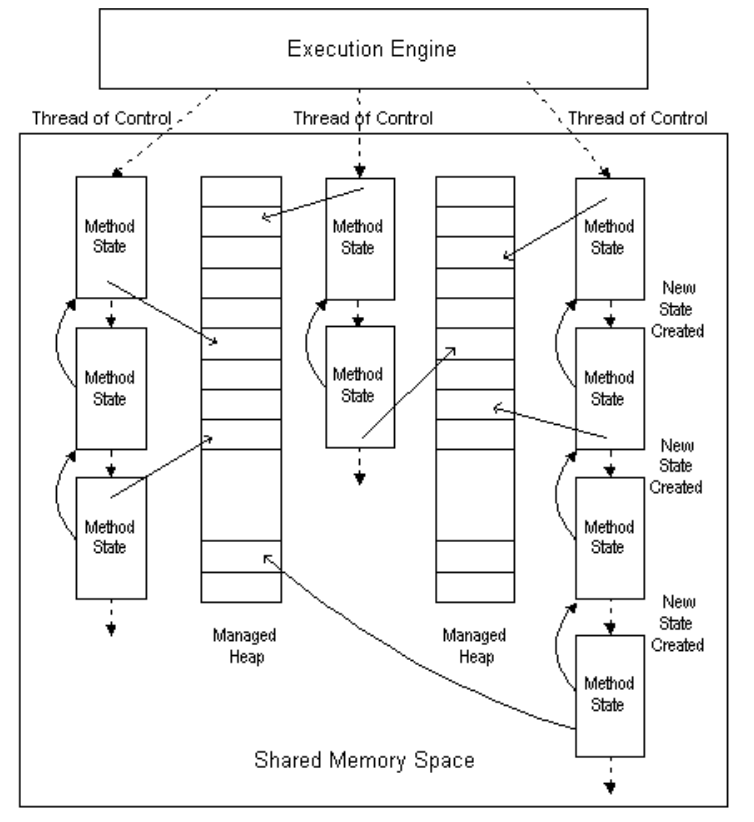
\includegraphics[width=3in,keepaspectratio]{ves}
    \centering
    \captionsetup{justification=centering}
    \caption{The structure of the VES and its nested method states, as represented by the ECMA standard~\cite{ecma335}.}
    \label{fig:ves}
\end{figure}

\subsubsection{Value storage}
The VES is not a ``true'' stack machine in the sense that all program information is stored on the stack;
rather, a method's stack is only a space to hold temporaries and set up arguments for method calls.
Instead, values are stored either in a method's declared local variables or within fields of an object.
These can be loaded onto the stack or stored from a stack value with the \texttt{ldarg}/\texttt{starg} and \texttt{ldfld}/\texttt{stfld}
CIL instructions.

At this point, the distinction between a full CLI value and a stack value becomes relevant.
While a CLI value can be an instance of an arbitrarily complex class or value type, a pointer, or a specific integer/floating-point type
(see section~\ref{sec:cts}),
the standard only requires that the evaluation stack support the following types as values:
\begin{itemize}
    \item 4-byte and 8-byte signed integers
    \item A pointer-sized signed integer
    \item A floating point value of unspecified precision
    \item Managed and unmanaged pointers (i.e., a pointer that references managed heap memory versus one known not to point into the heap)
    \item A GC-tracked reference to a CLI object
    \item User-defined value types
\end{itemize}
All other values are then transparently synthesized by the VES; for instance, a 1-byte integer will be zero-extended or sign-extended (as appropriate)
when loaded onto the stack, and CIL instructions that call specifically for 1-byte integers will have their arguments truncated.

\subsection{The Common Type System}\label{sec:cts}

\section{Implementation}

\subsection{Garbage collection with \texttt{gc-arena}}

\subsection{The call stack}

\subsection{CIL instructions}

\subsubsection{Unsafe operations}



\chapter{Conclusion}
\section{Technical evaluation}

\section{Developer experience}


% Format a LaTeX bibliography
\makebibliography

%\appendix
%
%\chapter{Extra Things I Chose to Include}
%\input{appendix}

% Figures and tables, if you decide to leave them to the end
%\input{figure}
%\input{table}

\end{document}
